\documentclass{article}

\usepackage{fancyhdr}
\usepackage{extramarks}
\usepackage{amsmath}
\usepackage{amsthm}
\usepackage{amsfonts}
\usepackage{tikz}
\usepackage[plain]{algorithm}
\usepackage{algpseudocode}
\usepackage{enumerate}
\usepackage{tikz,forest}
\usepackage{multicol}

\usetikzlibrary{arrows.meta}

\forestset{
    .style={
        for tree={
            base=bottom,
            child anchor=north,
            align=center,
            s sep+=1cm,
    straight edge/.style={
        edge path={\noexpand\path[\forestoption{edge},thick,-{Latex}] 
        (!u.parent anchor) -- (.child anchor);}
    },
    if n children={0}
        {tier=word, draw, thick, rectangle}
        {draw, diamond, thick, aspect=2},
    if n=1{%
        edge path={\noexpand\path[\forestoption{edge},thick,-{Latex}] 
        (!u.parent anchor) -| (.child anchor) node[pos=.2, above] {T};}
        }{
        edge path={\noexpand\path[\forestoption{edge},thick,-{Latex}] 
        (!u.parent anchor) -| (.child anchor) node[pos=.2, above] {F};}
        }
        }
    }
}

\usetikzlibrary{automata,positioning}

%
% Basic Document Settings
%

\topmargin=-0.45in
\evensidemargin=0in
\oddsidemargin=0in
\textwidth=6.5in
\textheight=9.0in
\headsep=0.25in

\linespread{1.1}

\pagestyle{fancy}
\lhead{\hmwkAuthorName}
\chead{\hmwkClass : \hmwkTitle}
\rhead{\firstxmark}
\lfoot{\lastxmark}
\cfoot{\thepage}

\renewcommand\headrulewidth{0.4pt}
\renewcommand\footrulewidth{0.4pt}

\setlength\parindent{0pt}

%
% Create Problem Sections
%

\newcommand{\enterProblemHeader}[1]{
    \nobreak\extramarks{}{Problem \arabic{#1} continued on next page\ldots}\nobreak{}
    \nobreak\extramarks{Problem \arabic{#1} (continued)}{Problem \arabic{#1} continued on next page\ldots}\nobreak{}
}

\newcommand{\exitProblemHeader}[1]{
    \nobreak\extramarks{Problem \arabic{#1} (continued)}{Problem \arabic{#1} continued on next page\ldots}\nobreak{}
    \stepcounter{#1}
    \nobreak\extramarks{Problem \arabic{#1}}{}\nobreak{}
}

\setcounter{secnumdepth}{0}
\newcounter{partCounter}
\newcounter{homeworkProblemCounter}
\setcounter{homeworkProblemCounter}{1}
\nobreak\extramarks{Problem \arabic{homeworkProblemCounter}}{}\nobreak{}

%
% Homework Problem Environment
%
% This environment takes an optional argument. When given, it will adjust the
% problem counter. This is useful for when the problems given for your
% assignment aren't sequential. See the last 3 problems of this template for an
% example.
%
\newenvironment{homeworkProblem}[1][-1]{
    \ifnum#1>0
        \setcounter{homeworkProblemCounter}{#1}
    \fi
    \section{Problem \arabic{homeworkProblemCounter}}
    \setcounter{partCounter}{1}
    \enterProblemHeader{homeworkProblemCounter}
}{
    \exitProblemHeader{homeworkProblemCounter}
}

%
% Homework Details
%   - Title
%   - Due date
%   - Class
%   - Section/Time
%   - Instructor
%   - Author
%

\newcommand{\hmwkTitle}{Problem Set\ \#1}
\newcommand{\hmwkDueDate}{September 15, 2017}
\newcommand{\hmwkClass}{CIS 520}
%\newcommand{\hmwkClassTime}{Section A}
\newcommand{\hmwkClassInstructor}{Lyle Ungar}
\newcommand{\hmwkAuthorName}{Eric Oh}

%
% Title Page
%

\title{
    \vspace{2in}
    \textmd{\textbf{\hmwkClass:\ \hmwkTitle}}\\
    \normalsize\vspace{0.1in}\small{Due\ on\ \hmwkDueDate\ }\\
    \vspace{0.1in}\large{\textit{\hmwkClassInstructor}}
    \vspace{3in}
}

\author{\textbf{\hmwkAuthorName}}
\date{}

\renewcommand{\part}[1]{\textbf{\large Part \Alph{partCounter}}\stepcounter{partCounter}\\}

%
% Various Helper Commands
%

% Useful for algorithms
\newcommand{\alg}[1]{\textsc{\bfseries \footnotesize #1}}

% For derivatives
\newcommand{\deriv}[1]{\frac{\mathrm{d}}{\mathrm{d}x} (#1)}

% For partial derivatives
\newcommand{\pderiv}[2]{\frac{\partial}{\partial #1} (#2)}

% Integral dx
\newcommand{\dx}{\mathrm{d}x}

% Alias for the Solution section header
\newcommand{\solution}{\textbf{\large Solution}}

% Probability commands: Expectation, Variance, Covariance, Bias
\newcommand{\E}{\mathrm{E}}
\newcommand{\Var}{\mathrm{Var}}
\newcommand{\Cov}{\mathrm{Cov}}
\newcommand{\Bias}{\mathrm{Bias}}

\begin{document}

\maketitle
\begin{center}
{\normalsize \noindent Collaborators: Jiarui Lu} \\
\end{center}
\pagebreak

\begin{homeworkProblem} 
High Dimensional Hi-Jinx

\solution

\begin{enumerate}

\item (Intra-class distance)
\begin{align*}
\E[(X-X')^2] &= \E[X^2-2XX'+X'^2] = E(X^2)-2E(XX')+E(X'^2) \\
&= (\sigma^2+\mu_1^2) -2\mu_1^2 + (\sigma^2+\mu_1^2) \\
&= 2\sigma^2
\end{align*}

\item (Inter-class distance)
\begin{align*}
\E[(X-X')^2] &= \E[X^2-2XX'+X'^2] = E(X^2)-2E(XX')+E(X'^2) \\
&= (\sigma^2+\mu_1^2) -2\mu_1\mu_2 + (\sigma^2+\mu_2^2) \\
&= (\mu_1-\mu_2)^2 + 2\sigma^2
\end{align*}

\item (Intra-class distance, m dimensions)
\begin{align*}
\E[\sum_{j=1}^m (X_j-X'_j)^2] &= \E[\sum_{j=1}^m (X_j^2 - 2 X_j X'_{j} + X'^2_j)] = \E[\sum_{j=1}^m X_j^2 - 2\sum_{j=1}^m X_j X'_j + \sum_{j=1}^m X'^2_j] \\
&= \sum_{j=1}^m \E(X_j^2)-2\sum_{j=1}^m \E(X_jX'_j) + \sum_{j=1}^m \E(X'^2_j) \\
&= \sum_{j=1}^m (\sigma^2+\mu_{1j}^2) - 2\sum_{j=1}^m(\mu_{1j}^2) + \sum_{j=1}^m (\sigma^2+\mu_{1j}^2) \\
&= 2m\sigma^2
\end{align*}

\item (Inter-class distance, m dimensions)
\begin{align*}
\E[\sum_{j=1}^m(X_j-X_j')^2] &= \E[\sum_{j=1}^m (X_j^2 - 2 X_j X'_{j} + X'^2_j)] = \E[\sum_{j=1}^m X_j^2 - 2\sum_{j=1}^m X_j X'_j + \sum_{j=1}^m X'^2_j] \\
&= \sum_{j=1}^m \E(X_j^2)-2\sum_{j=1}^m \E(X_jX'_j) + \sum_{j=1}^m \E(X'^2_j) \\
&= 2m\sigma^2 + \sum_{j=1}^m (\mu_{1j}-\mu_{2j})^2
\end{align*}

\item Under the assumption that only one dimension is informative about the class values, the ratio of expected intra-class distanced divided by inter-class distance is given by

\begin{equation*}
\frac{2m\sigma^2}{2m\sigma^2 + \sum_{j=1}^m (\mu_{1j}-\mu_{2j})^2} = \frac{2m\sigma^2}{2m\sigma^2 + (\mu_{11}-\mu_{21})^2}
\end{equation*}
where the equality follows from the assumption. Then as $m$ gets large, we have

\begin{align*}
lim_{m \rightarrow \infty} \frac{2m\sigma^2}{2m\sigma^2 + (\mu_{11}-\mu_{21})^2} = lim_{m \rightarrow \infty} \frac{2\sigma^2}{2\sigma^2} = 1
\end{align*}
where the first equality follows from L'Hopital's Rule. 
\end{enumerate}

\end{homeworkProblem}

\begin{homeworkProblem}

Non-Normal Norms

\solution

\begin{enumerate}

\item These are the distances to $x_1$ under the following norms:
\begin{itemize}

\item $L_0$
\begin{align*}
\lVert x_2-x_1 \rVert_0 = 2 \hspace{0.5in} \lVert x_3-x_1 \rVert_0 = 4 \hspace{0.5in} \lVert x_4-x_1 \rVert_0 = 4
\end{align*}
Thus, $x_2$ is the closest to $x_1$ under the $L_0$ norm. 

\item $L_1$
\begin{align*}
\lVert x_2-x_1 \rVert_1 = 5.4 \hspace{0.5in} \lVert x_3-x_1 \rVert_1 = 3.0 \hspace{0.5in} \lVert x_4-x_1 \rVert_1 = 3.3
\end{align*}
Thus, $x_3$ is the closest to $x_1$ under the $L_1$ norm. 

\item $L_2$
\begin{align*}
\lVert x_2-x_1 \rVert_2 = 4.8 \hspace{0.5in} \lVert x_3-x_1 \rVert_2 = 1.8 \hspace{0.5in} \lVert x_4-x_1 \rVert_2 = 1.9
\end{align*}
Thus, $x_3$ is the closest to $x_1$ under the $L_2$ norm. 

\item $L_{\mbox{inf}}$
\begin{align*}
\lVert x_2-x_1 \rVert_{\infty} = 4.7 \hspace{0.5in} \lVert x_3-x_1 \rVert_{\infty} = 1.5 \hspace{0.5in} \lVert x_4-x_1 \rVert_{\infty} = 1.4
\end{align*}
Thus, $x_4$ is the closest to $x_1$ under the $L_{\infty}$ norm. 

\end{itemize}

\item Below are the 1-Nearest Neighbor decision boundaries for the given norms. 

\begin{multicols}{2}
\begin{itemize}
\item $L_0$ \\
\includegraphics[width=0.35\textwidth]{images/L0.png}
\item $L_1$ \\
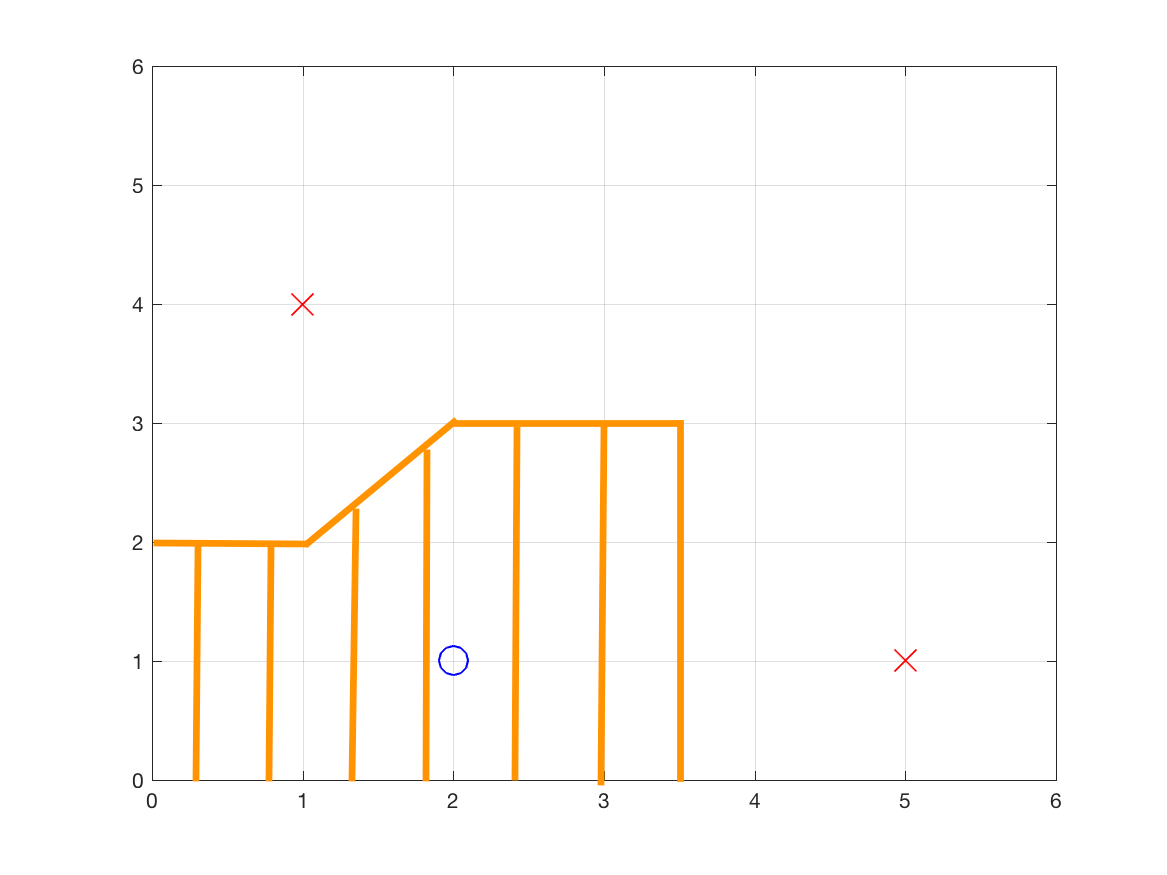
\includegraphics[width=0.35\textwidth]{images/L1.png}
\item $L_2$ \\
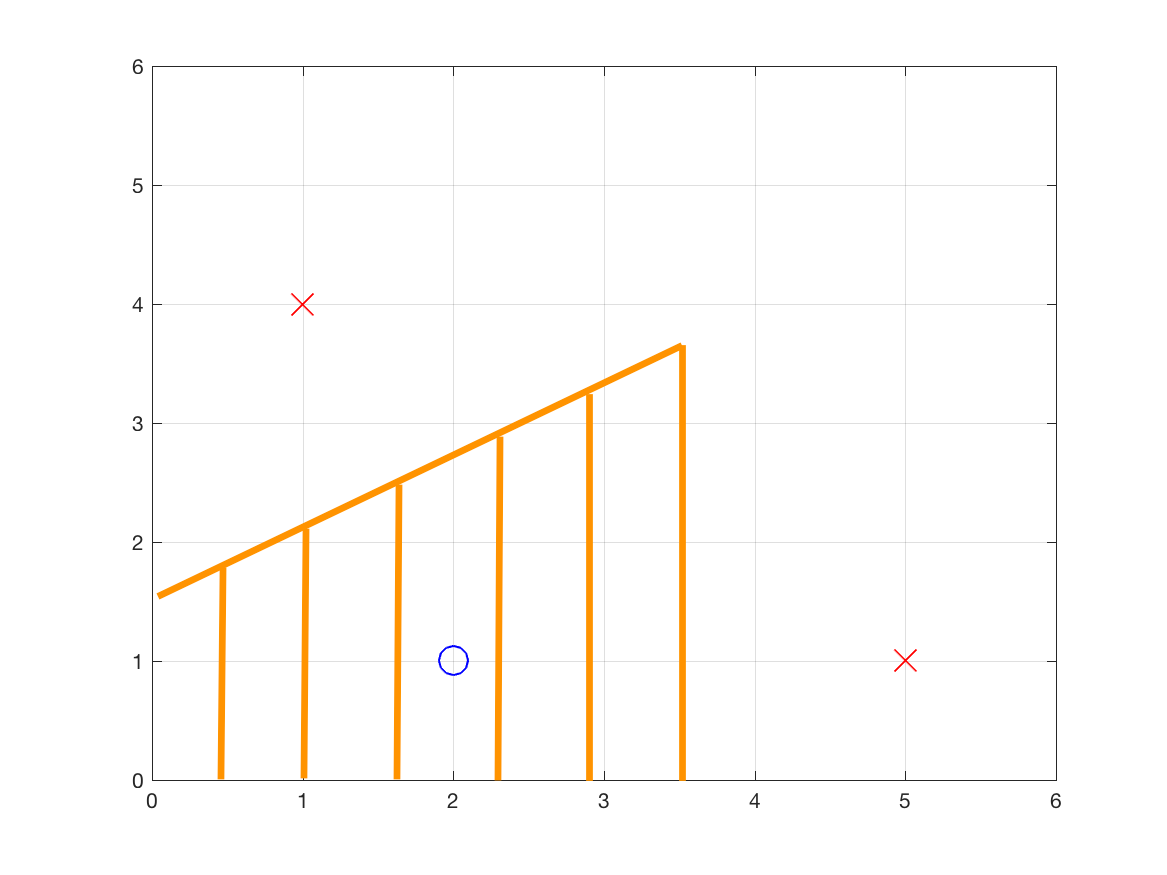
\includegraphics[width=0.35\textwidth]{images/L2.png}
\item $L_{\infty}$ \\
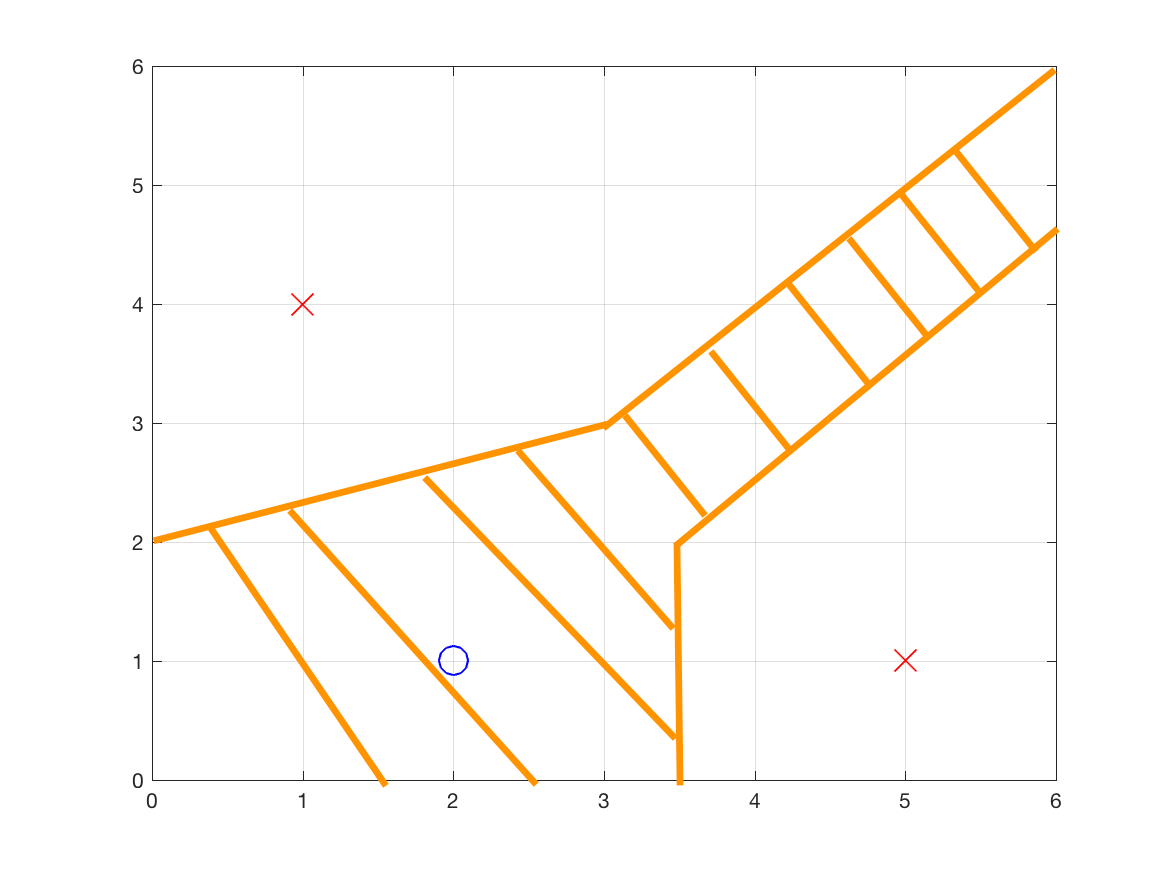
\includegraphics[width=0.35\textwidth]{images/Linf.png}
\end{itemize}
\end{multicols}
\end{enumerate}

\end{homeworkProblem}


%\begin{figure}
%\centering
%\includegraphics[width=0.4\textwidth]{L0.png}
%\end{figure}

\begin{homeworkProblem}

Conditional Independence in Probability Models

\solution

\begin{enumerate}

\item  The formula for $p(x_i)$ is given by
\begin{align*}
p(x_i) = \sum_j p(x_i, z_i=j) = \sum_j p(x_i|z_i=j)P(z_i=j) = \sum_j f_j(x_i)\pi_j
\end{align*}

\item The formula for $p(x_1,\ldots,x_n)$ is given by
\begin{align*}
p(x_1,\ldots,x_n) = \prod_{i=1}^n p(x_i) = \prod_{i=1}^n \sum_j f_j(x_i)\pi_j
\end{align*}
using the independence of $x_1,\ldots,x_n$. 

\item The formula for $p(z_u=v|x_1,\ldots,x_n)$ is given by
\begin{align*}
p(z_u=v|x_1,\ldots,x_n) = \frac{p(x_1,\ldots,x_n|z_u=v)p(z_u=v)}{p(x_1,\ldots,x_n)}
\end{align*}
using Bayes rule. We know that $p(z_u=v)= \pi_v$. Part 2 of this question gives the formula for the denominator. WLOG, assume $1<u<n$. Then the remaining term in the numerator is given by
\begin{align*}
p(x_1,\ldots,x_n|z_u=v) &= \prod_{i=1}^n p(x_i|z_u=v) = \prod_{i=1}^{u-1} p(x_i|z_u=v) \times p(x_u|z_u=v) \times \prod_{u+1}^n p(x_i|z_u=v) \\
&= \prod_{i=1}^{u-1} p(x_i) \times f_v(x_u) \times \prod_{u+1}^n p(x_i) \hspace{0.5in} \text{(By independence of $x_i$)} \\
&= \left(\prod_{i=1}^{u-1}\sum_j f_j(x_i)\pi_j\right) \times f_v(x_u) \times \left(\prod_{u+1}^n \sum_j f_j(x_i)\pi_j\right)
\end{align*}
Then it follows that
\begin{align*}
p(z_u=v|x_1,\ldots,x_n) &= \frac{\left(\prod_{i=1}^{u-1}\sum_j f_j(x_i)\pi_j\right) \times f_v(x_u) \times \left(\prod_{u+1}^n \sum_j f_j(x_i)\pi_j\right) \times \pi_v}{\prod_{i=1}^n \sum_j f_j(x_i)\pi_j} \\
&= \frac{f_v(x_u)\pi_v}{\sum_j f_j(x_u)\pi_j}
\end{align*}
\end{enumerate}
\end{homeworkProblem}


\begin{homeworkProblem}

Fitting distributions with KL divergence

\solution

\begin{enumerate}

\item The KL divergence between two univariate Gaussian distributions $p(x) \sim \mbox{N}(\mu_1,\sigma^2)$ and $q(x) \sim \mbox{N}(\mu_2,1)$ is given by
\begin{align*}
KL(p(x) \lVert q(x)) &= \E_p\left[\log \frac{p(x)}{q(x)} \right] = \E_p \left[\log \left\{ \frac{\sqrt{2\pi}}{\sqrt{2\pi\sigma^2}} \exp\left(-\frac{1}{2\sigma^2}(x-\mu_1)^2 + \frac{1}{2}(x-\mu_2)^2\right)\right\}\right] \\
&= \E_p \left[\log(\sigma^{-1}) + \left\{-\frac{1}{2\sigma^2}(x-\mu_1)^2 + \frac{1}{2}(x-\mu_2)^2\right\} \right] \\
&= \log(\sigma^{-1}) + \E_p \left[-\frac{1}{2\sigma^2}(x-\mu_1)^2 + \frac{1}{2}(x-\mu_2)^2\right] \\
&= g(\sigma) + \E_p\left[f(x,\mu_1,\mu_2,\sigma)\right]
\end{align*}
where $f(x,\mu_1,\mu_2,\sigma)=-\frac{1}{2\sigma^2}(x-\mu_1)^2 + \frac{1}{2}(x-\mu_2)^2$ and $g(\sigma)=\log(\sigma^{-1})$. 

\item For fixed $\mu_2$ and $\sigma$, the value of $\mu_1$ that minimizes $KL(p(x)\lVert q(x))$ is found by taking the derivative of the expression in Part 1 w.r.t $\mu_1$.
\begin{align*}
KL(p(x) \lVert q(x)) &= \E_p \left[-\frac{1}{2\sigma^2}(x-\mu_1)^2 + \frac{1}{2}(x-\mu_2)^2\right] + \log(\sigma^{-1}) = -\frac{1}{2\sigma^2}\E(x-\mu_1)^2 + \frac{1}{2}\E(x-\mu_2)^2 + \log(\sigma^{-1}) \\
&= -\frac{\sigma^2}{2\sigma^2} + \frac{1}{2}\E\left(x-\mu_1+\mu_1-\mu_2\right)^2 + \log(\sigma^{-1}) \\
&= -\frac{1}{2} + \frac{1}{2}\E\left( (x-\mu_1)^2 + 2(x-\mu_1)(\mu_1-\mu_2) + (\mu_1-\mu_2)^2\right) + \log(\sigma^{-1}) \\
&= -\frac{1}{2} + \frac{1}{2}\left[\E(x-\mu_1)^2 + 2\E(x-\mu_1)(\mu_1-\mu_2) + \E(\mu_1-\mu_2)^2\right] + \log(\sigma^{-1}) \\ 
&= -\frac{1}{2} + \frac{1}{2}\left[\sigma^2 + (\mu_1-\mu_2)^2\right] + \log(\sigma^{-1}) \hspace{0.5in} \text{(Middle term above is 0)} \\
\frac{d}{d\mu_1}KL(p(x) \lVert q(x)) &= \mu_1-\mu_2 \equiv 0 \hspace{0.2in} \Rightarrow \hspace{0.2in} \mu_1 = \mu_2  \\
\end{align*}
Thus, setting $\mu_1$ equal to $\mu_2$ minimizes $KL(p(x) \lVert q(x))$ for fixed $\mu_2$ and $\sigma$. At this minimum, the value is $-\frac{1}{2} + \frac{\sigma^2}{2} + \log(\sigma^{-1})$. 
\end{enumerate}
\end{homeworkProblem}

\begin{homeworkProblem}

Decision Trees

\solution

\begin{enumerate}

\item The sample entropy $H(Y)$ for this training data is given by
\begin{align*}
H(Y) = -\left[P(Y=+)\log(P(Y=+)) + P(Y=-)\log(P(Y=-))\right]=-\left[\frac{13}{25}\log\left(\frac{13}{25}\right) + \frac{12}{25}\log\left(\frac{12}{25}\right)\right]=0.9988
\end{align*}

\item The conditional entropies $H(Y|X_1)$ and $H(Y|X_2)$ are given by
\begin{align*}
H(Y|X_1)&=P(X_1=T)H(Y|X_1=T) + P(X_1=F)H(Y|X_1=F) \\
&= \frac{11}{25}\left[-\left\{\frac{4}{11}\log\left(\frac{4}{11}\right)+\frac{7}{11}\log\left(\frac{7}{11}\right)\right\}\right] + \frac{14}{25}\left[-\left\{\frac{9}{14}\log\left(\frac{9}{14}\right)+\frac{5}{14}\log\left(\frac{5}{14}\right)\right\}\right] \\
&= 0.9427
\end{align*}
and
\begin{align*}
H(Y|X_2)&=P(X_2=T)H(Y|X_2=T) + P(X_2=F)H(Y|X_2=F) \\
&= \frac{11}{25}\left[-\left\{\frac{5}{11}\log\left(\frac{5}{11}\right)+\frac{6}{11}\log\left(\frac{6}{11}\right)\right\}\right] + \frac{14}{25}\left[-\left\{\frac{8}{14}\log\left(\frac{8}{14}\right)+\frac{6}{14}\log\left(\frac{6}{14}\right)\right\}\right] \\
&= 0.9891
\end{align*}
Thus the information gains are 
\begin{align*}
IG(X_1)=H(Y)-H(Y|X_1)=.0561 \hspace{0.3in} IG(X_2)=H(Y)-H(Y|X_2)=.0097
\end{align*}

\item The decision tree learned by ID3 is given by 
\begin{center}
\begin{forest} 
[$X_1$, tikz={\draw[{Latex}-, thick] (.north) --++ (0,1);}
    [$X_2$
        [-] 
        [+] 
    ]   
    [$X_2$
        [+]   
        [+] 
    ]   
] 
\end{forest}
\end{center}

\item If variables $X$ and $Y$ are independent, then $IG(x,y)=0$. We prove this by using the definition of independence given by $p(x,y)=p(x)p(y)$ in the KL-divergence information gain. 
\begin{align*}
IG(x,y) \equiv KL(p(x)\lVert q(x)) &= -\sum_x \sum_y p(x,y) \log\left(\frac{p(x)p(y)}{p(x,y)}\right) \\
&= -\sum_x \sum_y p(x,y) \log\left(\frac{p(x)p(y)}{p(x)p(y)}\right) \\
&= -\sum_x \sum_y p(x,y) \times 0 \\
&= 0
\end{align*}

\item We can show that the definition of information gain using the KL divergence is equivalent to the definition involving entropy, ie. $IG(x,y)=H(x)-H(x|y)=H(y)-H(y|x)$. We first show that $IG(x,y)=H(y)-H(y|x)$.
\begin{align*}
IG(x,y) &= -\sum_x \sum_y p(x,y) \log\left(\frac{p(x)p(y)}{p(x,y)}\right) = -\sum_x \sum_y p(y|x)p(x)\log\left(\frac{p(x)p(y)}{p(y|x)p(x)}\right) \\
&= -\sum_x p(x) \sum_y p(y|x) \left\{\log(p(y)) - \log(p(y|x))\right\} \\
&= -\sum_x \sum_y p(x,y)\log(p(y)) + \sum_x p(x) \sum_y p(y|x)\log(p(y|x)) \\
&= -\sum_y \sum_x p(x,y)\log(p(y)) - \sum_x p(x) H(Y|X=x) \\
&= -\sum_y p(y)\log(p(y)) - \sum_x p(x) H(Y|X=x) \\
&= H(Y) - H(Y|X)
\end{align*}
Note that we could have chosen to write $p(x,y)=p(x|y)p(y)$ in the first line of the proof, giving us
\begin{align*}
IG(x,y) &= -\sum_x \sum_y p(x,y) \log\left(\frac{p(x)p(y)}{p(x,y)}\right) = -\sum_x \sum_y p(x|y)p(y)\log\left(\frac{p(x)p(y)}{p(x|y)p(y)}\right) \\
\end{align*}
The proof then follows by symmetry and we have shown that $IG(x,y)=H(x)-H(x|y)$. To show that $H(x)-H(x|y)=H(y)-H(y|x)$, it suffices to show that 
\begin{align*}
-\sum_x \sum_y p(y|x)p(x)\log\left(\frac{p(x)p(y)}{p(y|x)p(x)}\right) = -\sum_x \sum_y p(x|y)p(y)\log\left(\frac{p(x)p(y)}{p(x|y)p(y)}\right)
\end{align*}
Bayes rule gives us $p(y|x)p(x)=p(x|y)p(y)$, so the above equality follows immediately.  \\
\\
Note, the above proof can also be done using continuous $x$ and $y$. In this case, the sums are replaced by integrals and we would need to invoke Fubini's Theorem to change the order of integration. Checking the conditions for Fubini's Theorem is beyond the scope of this class; thus, the rest of the proof would follow as is. 
\end{enumerate}

\end{homeworkProblem}




\end{document}
